\documentclass[border=10pt]{standalone}
\usepackage[svgnames]{xcolor}
\usepackage{amsmath}
\usepackage{pgfplots}
\pgfplotsset{compat=newest}
\usepackage[sfdefault]{FiraSans}
\usepackage{FiraMono}
\renewcommand*\familydefault{\sfdefault}
\begin{document}
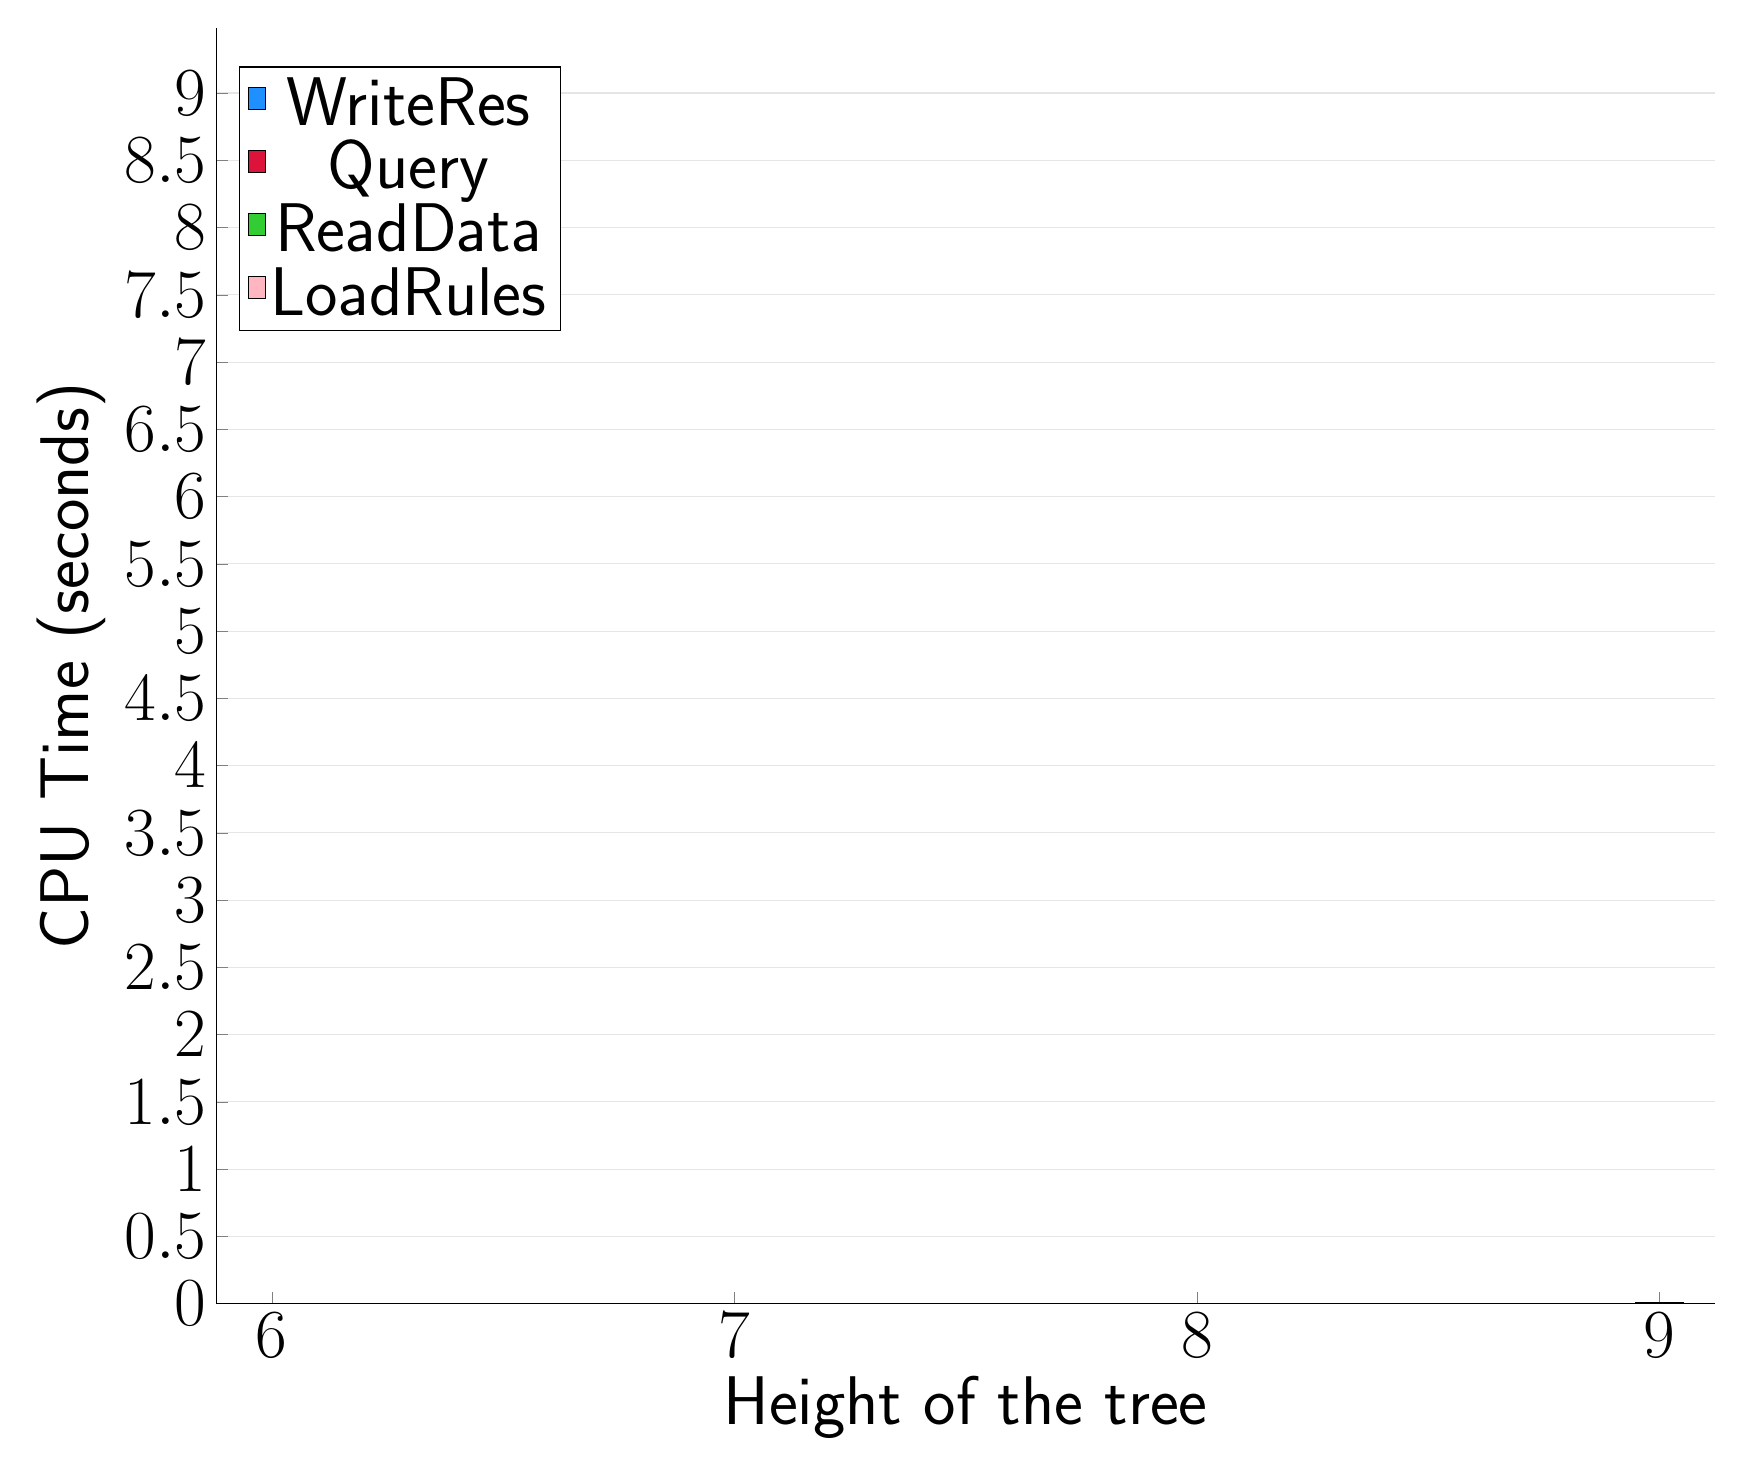
\begin{tikzpicture}
\begin{axis}[
   ybar stacked,
   width=1.7\textwidth,
   bar width=0.6cm,
   ymajorgrids, tick align=inside,
   major grid style={draw=gray!20},
   xtick=data,
   ymin=0, ymax=9.482,
   axis x line*=bottom,
   axis y line*=left,
   enlarge x limits=0.04,
   legend style={
       at={(0.23, 0.97)},
       anchor=north east,
       legend columns=1,
       font=\Huge,
   },
   ylabel={CPU Time (seconds)},
   xlabel={Height of the tree},
   label style={font=\Huge},
   tick label style={font=\Huge},
]
\addlegendimage{fill=DodgerBlue, draw=black, line width=0.2pt}
\addlegendentry{WriteRes}
\addlegendimage{fill=Crimson, draw=black, line width=0.2pt}
\addlegendentry{Query}
\addlegendimage{fill=LimeGreen, draw=black, line width=0.2pt}
\addlegendentry{ReadData}
\addlegendimage{fill=LightPink, draw=black, line width=0.2pt}
\addlegendentry{LoadRules}
\addplot +[fill=LightPink, draw=black, line width=0.55pt] coordinates {
(6, 0.0005512000000000002)
(7, 0.000549)
(8, 0.0005482000000000004)
(8, 0.0005459999999999999)
(8, 0.0005478000000000002)
(9, 0.0005475999999999998)
(9, 0.0005479999999999993)
(9, 0.0005549999999999999)
(9, 0.0005471999999999993)
(9, 0.0005483999999999999)
};
\addplot +[fill=LimeGreen, draw=black, line width=0.55pt] coordinates {
(6, 0.0001665999999999996)
(7, 0.0002186)
(8, 0.00031699999999999963)
(8, 0.0003145999999999998)
(8, 0.00031800000000000025)
(9, 0.0005156000000000003)
(9, 0.0005172000000000002)
(9, 0.0005200000000000006)
(9, 0.0005184000000000007)
(9, 0.0005166000000000004)
};
\addplot +[fill=Crimson, draw=black, line width=0.55pt] coordinates {
(6, 4.539999999999996e-05)
(7, 9.220000000000026e-05)
(8, 0.00019480000000000002)
(8, 0.0001953999999999998)
(8, 0.000195)
(9, 0.00042959999999999976)
(9, 0.000429)
(9, 0.00043360000000000024)
(9, 0.0004282000000000002)
(9, 0.000428)
};
\addplot +[fill=DodgerBlue, draw=black, line width=0.55pt] coordinates {
(6, 0.00027580000000000004)
(7, 0.0006028000000000001)
(8, 0.0013511999999999999)
(8, 0.0013700000000000001)
(8, 0.0013871999999999999)
(9, 0.0030614)
(9, 0.0030759999999999997)
(9, 0.0030941999999999996)
(9, 0.00307)
(9, 0.0030648000000000003)
};
\end{axis}
\end{tikzpicture}

\end{document}
